
\chapter{Fundamentação Teórica}
\label{chap:fundamentacao}

Neste capítulo, são apresentados os conceitos que servem de insumo para a elaboração das etapas seguintes desse trabalho. Na seção \ref{sec:complexidade} são demostrados alguns conceitos necessários para identificar e classificar a complexidade de um algoritmo. A seção \ref{sec:pd} explica o básico sobre programação dinâmica, seus principais termos e o conceito de otimização, que servirá de base para a elaboração dos capítulos seguintes. Por fim, no capítulo \ref{sec:ensino} é feita uma análise de alguns trabalhos relacionados com o ensino de programação.



\section{Complexidade de Algoritmos}
\label{sec:complexidade}
Na ciência da computação, analisar um algoritmo está relacionado com a identificação da quantidade de recursos necessários para sua execução, podendo ser a quantidade de memória utilizada, largura de banda de comunicação, hardware do computador. Porém mais frequentemente a preocupação maior é em se medir o tempo computacional gasto para realizar determinado código \cite{Cormen09a}.

Quando é feita a análise de complexidade, é possível identificar qual classe um determinado algoritmo pertence. A tabela \ref{tab:classes} lista algumas classes de forma ordenada, sendo a primeira função a melhor possível e a última a pior. Após classificar um algoritmo, é possível escolher entre diversas soluções para um mesmo problema, qual é a mais adequada no momento e poder saber antes de executar quanto tempo e memória o algoritmo irá gastar quando o tamanho da entrada for $n$, onde $n$ corresponde, geralmente a quantidade de elementos que devem processados. Na figura \ref{fig:complexity} é possível observar o comportamento de algumas funções na medida que a quantidade de elementos aumenta.


\begin{table}[H]
	\centering
	\caption[Principais classes de funções para analisar algoritmos]{Principais classes de funções para analisar algoritmos}
	\label{tab:classes}
	\begin{tabular}{c|c}
		\hline \SPACE
		\textbf{Notação} & \textbf{Exemplo de algoritmos} \\ \hline \SPACE
		$O(1)$ & Determinar se um número é par ou ímpar \\ \hline \SPACE
		$O(log n)$ & Busca binária \\ \hline \SPACE
		$O(\sqrt{n})$ & Determinar se um número é primo \\ \hline \SPACE
		$O(n)$ & Procurar um elemento em um \textit{array} não ordenado \\ \hline \SPACE
		$O(n * log n)$ & \textit{Merge sort}\protect\footnotemark \\ \hline \SPACE
		$O(n^2)$ & \textit{Bubble sort}\protect\footnotemark \\ \hline \SPACE
		$O(n^3)$ & \textit{Floyd-Warshall}\protect\footnotemark \\ \hline \SPACE
		$O(n^c)$ & Encontrar o maior emparelhamento em um grafo \\ \hline \SPACE
		$O(c^n)_{c > 1}$ & Resolver o problema do caixeiro viajante\protect\footnotemark com programação dinâmica \\ \hline \SPACE
		$O(n!)$ & Resolver o problema do caixeiro viajante com força bruta \\ \hline
	\end{tabular}

	\fonte{Pr\'oprio Autor.}
\end{table}
\addtocounter{footnote}{-3}
\footnotetext{Ver mais em: http://quiz.geeksforgeeks.org/merge-sort/}
\addtocounter{footnote}{1}
\footnotetext{Ver mais em: http://quiz.geeksforgeeks.org/bubble-sort/}
\addtocounter{footnote}{1}
\footnotetext{Ver mais em: http://www.geeksforgeeks.org/dynamic-programming-set-16-floyd-warshall-algorithm/}
\addtocounter{footnote}{1}
\footnotetext{Ver mais em: http://www.geeksforgeeks.org/travelling-salesman-problem-set-1/}

\begin{figure}[H]
	\centering
	\caption[Gráfico das principais classes de complexidade]{Gráfico das principais classes de complexidade}
	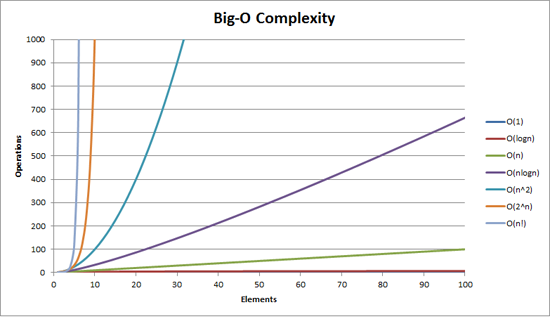
\includegraphics[width=0.7\textwidth]{complexity.png} % <- formatos PNG, JPG e PDF
	\fonte{PERRETT, 2010\nocite{Perrett2010}}
	\label{fig:complexity}
\end{figure}

\section{Programação dinâmica}
\label{sec:pd}

Programação dinâmica é uma técnica que combina soluções de subproblemas, da mesma maneira que a divisão e conquista, que divide o problema em subproblemas, resolve cada um recursivamente e depois é feita a junção das soluções para resolver o problema original. Porém este método é normalmente utilizado quando os subproblemas se sobrepõem, ou seja, um mesmo estado é encontrado diversas vezes na etapa de divisão. Portanto, se fosse aplicado um algoritmo ingênuo de divisão e conquista, um mesmo estado seria resolvido várias vezes, aumentando o custo computacional do algoritmo \cite{Cormen09a}. 

Para resolver o problema de sobreposição, a técnica de programação dinâmica salva a resposta de todos os estados que vão sendo encontrados. Assim, no momento que se deparar com algo que já foi resolvido ela simplesmente retorna o valor que já estava armazenado. 

A sequência de Fibonacci é um exemplo de fácil entendimento de quando é necessário a utilização de programação dinâmica. Esta é uma sequência de números inteiros que tem seu início com 0 e 1, os termos subsequentes são uma soma dos dois últimos números. A sequência recebeu o nome do matemático Leonardo de Pisa, mais conhecido como Fibonacci, que no ano de 1202 descreveu o crescimento da população de coelhos utilizando esta sequência \cite{LiveScience2013}. Os primeiros termos são:
\begin{equation}
0, 1, 1, 2, 3, 5, 8, 13, 21, 34, 55, 89, 144, 233, 377, 610, ...
\label{eq:fib}
\end{equation}
podendo ser representada através da seguinte recorrência, onde $fib(i)$ representa $i$-ésimo termo da sequência:
\begin{equation}
fib(i)=
\begin{cases}
i &\text{se } i \leq{1},\\
fib(i - 1) + fib(i - 2) &\text{se } i > {1}.
\end{cases}
\label{eq:fibrecorrence}
\end{equation}

\begin{figure}[H]
	\centering
	\caption[Árvore de recursão do Fibonacci de 5]{Árvore de recursão do Fibonacci de 5}
	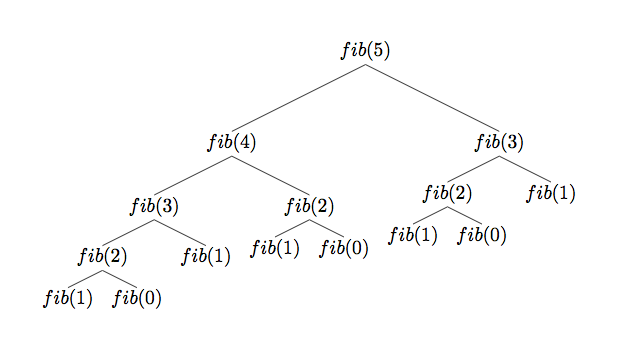
\includegraphics[width=0.7\textwidth]{fib5.png} % <- formatos PNG, JPG e PDF
	\fonte{SCHWARTZ, 2011\nocite{Schwartz2011}}
	\label{fig:fib5}
\end{figure}


Na figura \ref{fig:fib5} é apresentada a árvore de recursão gerada ao utilizar a equação \ref{eq:fibrecorrence} para o cálculo do $fib(5)$. Através dela, é fácil ver que diversos estados estão se repetindo, por exemplo: $fib(2)$ aparece três vezes e sempre que é encontrado ele é divido no $fib(1)$ e $fib(0)$, assim deixando a  complexidade deste algoritmo em $O(2^{N})$. Ao aplicar programação dinâmica neste algoritmo é possível reduzir a complexidade para $O(N)$, pois cada estado será expandido uma única vez.

O código a seguir mostra como seria a implementação da função sem a utilização de programação dinâmica.
\begin{lstlisting}[caption={Implementação Fibonacci sem programação dinâmica},label={lst:fibsimples}]
int fib(int i){
	if(i <= 1)
		return i;
	return fib(i - 1) + fib(i - 2);
}

\end{lstlisting}

Para otimizar o código e utilizar programação dinâmica basta incluir uma tabela que salva todos os estados. Sua inclusão faz uma alteração mínima no código, como é mostrado no algoritmo \ref{lst:fibpd}.


\begin{lstlisting}[caption={Implementação Fibonacci com programação dinâmica},label={lst:fibpd}]
#define MAX 20 
int tabela[MAX + 1]; 
					 					 
int fib(int i){
	if(tabela[i] != -1) 
		return tabela[i];
	if(i <= 1)
		return tabela[i] = i;
	return tabela[i] = fib(i - 1) + fib(i - 2);
}
\end{lstlisting}

Para mais informações sobre programação dinâmica e suas técnicas, o site \textit{TopCoder}\footnote{https://www.topcoder.com/community/data-science/data-science-tutorials/} possui um artigo amplo com vários problemas e dicas para soluções. Ele divide sua explicação em teoria e prática, começando nos tópicos mais simples e indo até alguns mais avançados.

\subsection{Otimizações}

Ao utilizar programação dinâmica para otimizar um problema, normalmente ocorre uma queda drástica na classe de complexidade associada a solução, como é o caso da sequência de Fibonacci, discutida na seção \ref{sec:pd}, onde foi possível sair de uma complexidade exponencial para uma linear. Apesar de parecer uma ótima forma de solucionar um problema, às vezes apenas aplicar programação dinâmica não é suficiente, e existem casos onde é possível e necessário otimizar ainda mais.

Para utilizar uma técnica de otimização de programação dinâmica, alguns critérios em relação a função de recorrência devem ser correspondidos. Cada técnica tem uma abordagem que possibilita a resolução de um conjunto de problemas que compartilham certas propriedades.

A tabela \ref{tab:otimizacoes} ilustra algumas formas otimizações existentes, que possibilitam tanto na redução de espaço, quanto de tempo. Estas técnicas serão discutidas no capítulo \ref{chap:desenvolvimento}.

\begin{table}[H]
	\centering
	\caption[Otimizações de programação dinâmica]{Otimizações de programação dinâmica}
	\label{tab:otimizacoes}
	\begin{tabular}{p{4cm} | p{11cm}}
		\hline \SPACE
		\textbf{Nome/Tipo} & \textbf{Característica} \\ \hline \SPACE
		Redução de espaço &  Reduz a quantidade de memória necessária quando um estado depende de uma quantidade fixa de outros estados \\ \hline \SPACE
		Estrutura de dados &  Reduz a complexidade de tempo com o auxílio de uma estrutura de dados que consegue responder a consultas do tipo mínimo ou máximo em um intervalo de uma \textit{array}  \\ \hline \SPACE
		\textit{Divide and Conquer} & Realiza divisão e conquista para encontrar o ponto ótimo necessário para se resolver o estado atual, reduzindo a complexidade temporal \\ \hline \SPACE
		\textit{Knuth Optimization} & Utiliza informações de onde estava a solução ótima de um estado anterior para diminuir o espaço de busca dos outros, assim reduzindo a complexidade temporal  \\ \hline \SPACE
		\textit{Convex Hull Trick} & Através de conceitos geométricos, essa técnica possibilita a redução da complexidade temporal \\ \hline 
	\end{tabular}
	
	\fonte{Pr\'oprio Autor.}
\end{table}

\section{Ensino de algoritmos}
\label{sec:ensino}

O ensino de algoritmos, por se tratar de assuntos que normalmente não são tão simples, com um fundamentação matemática extensa, não é uma tarefa fácil, portanto foi feita uma busca na literatura de trabalhos que têm por objetivo criar uma metodologia de ensino. Assim servindo de modelo para o que está aqui sendo desenvolvido.


\nocite{methods}
Szlávi e Zsakó (2003) apresentaram diversas metodologias relacionadas ao ensino de programação. O autor discuti sobre alguns modelos e exemplifica quando e para qual nível de estudante cada método será mais proveitoso ao ser aplicado. Estes métodos determinam a forma de estruturar o curso que deseja ser ensinado e a maneira de explicar os conteúdos.

\nocite{doi:10.1076/csed.13.2.137.14200} 
Uma ampla pesquisa na literatura com o foco na parte educacional do estudo de programação foi feita. Diversos métodos e tópicos foram identificados e analisados para poder ser realizado uma classificação, e assim, auxiliar os professores a identificar em seus alunos características comuns e padrões, que poderão ser contornados com base no que já foi realizado e está documentado na literatura, é mostrado por Robins, Rountree (2003).

\nocite{Pears:2007:SLT:1345443.1345441}
Pears \textit{et al.} (2007) desenvolveu um \textit{survey} que reúne algumas formas da literatura de ensinar a introdução de programação. Além disso, os trabalhos reunidos, foram classificados e agrupados pela forma de ensino e pelos métodos aplicados.


\nocite{teachingapplications} 
Zsakó e Nóra (2008) realizaram uma análise nos principais métodos e aplicações que auxiliam no aprendizado e no ensino dos tópicos de\sigla{ICT}{Information and Communication Technology}(do inglês, \textit{Information and Communication Technology}). Para cada método é exemplificado o seu funcionamento, como realizar a sua aplicação e para qual nível de estudante ele é mais apropriado. 


\nocite{teachingapplicationslanguages} 
No trabalho desenvolvido por Papp-varga, Szlávi e Zsakó (2008), foi feita uma análise semelhante a que foi realizada no trabalho apresentado na subseção anterior. Porém, o foco deste é o ensino de uma linguagem de programação, portanto os métodos apresentados demostram os passos ideais para transmitir os conceitos da linguagem proposta.

\nocite{newapproach} 
Radošević, Orehovački e Lovrenčić (2009), se propõem em criar uma ferramenta que facilite o aprendizado de linguagens de programação básicas, como C++, ao invés da utilização de\sigla{IDE}{Integrated Development Environment}(do inglês, \textit{Integrated Development Environment}). A finalidade desta ferramenta é ajudar os estudantes em não cometer erros que são comuns a quem está iniciando. Além disso, oferecer uma forma mais simples do professor auxiliar seus alunos.

\nocite{Vihavainen:2011:EAM:1953163.1953196}
Vihavainen, Paksula e Luukkainen (2011), discutem como ensinar o básico de programação para quem está começando. O autor propõe um modelo de ensino e faz a aplicação deste em uma turma de um curso de ciência da computação. Ao final do trabalho é feito um comparativo entre uma turma que utilizou da metodologia proposta e uma que não usou, e os resultados foram positivos, mostrando que a quantidade de evasão e reprovação foram reduzidos.

Apesar de existirem diversos trabalhos que tratam sobre o ensino de algoritmos e programação, todos os encontrados têm um foco para um nível básico de conhecimento, levando em conta alunos que estão iniciando nesta área, portanto, não será aplicado nenhum deste diretamente. No capítulo \ref{chap:metodo} será discutido a metodologia elaborada para a construção do trabalho.
 



